% 来源: 19c9fbd0-f1d2-808a-8000-0000b4a1e732_1.5_端_定时器.pdf
% 提取时间: 2026-02-28T22:51:53+08:00

1.5 端：定时器
第7章 定时器维护
“过去如是，现在如是，将来亦如是：时光之轮永不停歇。”——罗伯特·勃朗宁
系统中的定时器模块就好比是一位秘书，负责记录忙碌主管的所有日程安排。主管告知秘书安排日程，
有时还会要求在日程开始前取消安排。秘书的工作是在日程即将开始前提醒主管。实际上，许多秘书会
使用所谓的“到期提醒文件”来完成这项工作，这是一个涵盖未来N天的动态窗口。当一天的日程结束后，
到期提醒文件会滚动更新，跳过当天。我们会发现到期提醒文件和本章的主要数据结构——时间轮有很
强的相似性。
本章内容安排如下：7.1节描述了为什么需要定时器；7.2节介绍了定时器例程的模型以及对性能至关重要
的相关参数；7.3节讲述了维护定时器的最简单技术，其中一些在某些情况下仍然适用；7.4节引入了主要
数据结构——时间轮，随后在7.5节和7.6节分别介绍了时间轮的两种具体实例：哈希轮和分层时间轮；本
章最后在7.9节介绍了一种称为软定时器的技术，它通过在其他系统调用中分摊定时器维护开销来降低定
时器的开销。表7.1总结了各种定时器方案中应用的原理。
与第一版相比，最显著的变化可能是如今云主机中经常使用成千上万的细粒度定时器（Saeed等人，
2017）。这些定时器通过流量整形为虚拟机流量提供带宽隔离，并且用于像BBR（Cardwell等人，
2017）这样的现代拥塞控制算法中，BBR算法通过精细的速率调整来减少数据包丢失。这些新应用更有
力地证明了使用本章主要数据结构（时间轮）的必要性，以及在多核机器中实现更精简定时器的需求。
快速参考指南
对于实现者而言，最有用的部分可能是7.5节关于哈希时间轮的内容。哈希时间轮的多个版本已出现在许
多操作系统中，例如FreeBSD，以及在谷歌机器中作为Carousel（Saeed等人，2017）流量整形软件的
一部分。Linux早期版本以及最近一个版本使用分层时间轮（7.6节），这个版本效率更高，但定时器精
度较低（Corbet，2015）。
 序号                原理                   定时器技术
 P14               使用数组存储有界定时器          基本时间轮
 P2c, 4            利用每日时间更新             /
 P15               使用哈希或分层结构            哈希、分层时间轮
 P10               传递句柄以删除定时器           任何定时器方案
 P4                利用系统调用等              软定时器

                                                       1
P3                 放宽对精确定时器的需求       /
P11                优化快速定时器           /

7.1 为什么需要定时器？
系统为什么需要定时器呢？系统需要定时器来进行故障恢复，同时也用于实现一些算法，在这些算法
中，时间或相对时间的概念是不可或缺的。有几种类型的故障无法异步检测到。有些故障可以通过定期
检查来发现（例如，磁盘看门狗定时器），这类定时器总是会到期。而其他一些故障只能通过在指定时
间内没有某些积极动作（例如，消息确认）来推断。如果故障很少发生，这些定时器很少会到期。
许多系统还会实现使用时间或相对时间的算法。例如，控制某些实体产生速率的算法（如网络中的基于
速率的流量控制）和调度算法。这些定时器几乎总是会到期。
当出现以下任何一种情况时，实现定时器模块的算法性能就会成为一个问题。首先，如果该算法由一个
处理器实现，并且每次硬件时钟滴答时处理器都会被中断，且中断开销很大，那么性能就会成为问题。
其次，如果需要细粒度的定时器，性能也会成为问题。第三，如果活动定时器的平均数量很大，性能同
样会成为问题。在运行速度为100 Gbps、对成千上万的流量进行精细流量整形的云服务器中，这三个因
素正变得越来越关键（Saeed等人，2017）。
如果硬件时钟每次滴答都中断主机，且滴答之间的间隔在微秒量级，那么中断开销是相当大的。大多数
主机操作系统提供的定时器粒度较粗（毫秒或秒）。或者，在某些系统中，更细粒度的定时器存在于专
用硬件中。在这两种情况下，定时器算法的性能都会是一个问题，因为它们决定了启动或停止定时器所
产生的延迟以及可以同时存在的定时器数量。
例如，考虑分布式系统中成员之间的通信。由于消息可能在底层网络中丢失，因此在某种程度上需要定
时器来触发重传。分布式系统中的一个主机可能有多个未完成的定时器。例如，一台有50,000个连接的
服务器，每个连接有三个定时器。此外，随着网络速度提升到100吉比特及更高，所需的定时器分辨率以
及启动和停止定时器的频率都会增加。
一些网络实现并不是为每个数据包都使用一个定时器，而是整个网络包只使用几个定时器。例如，TCP
实现通过为所有未完成的数据包维护自己的定时器，并使用单个内核定时器作为时钟来运行这些定时
器，从而仅用两个定时器就解决了问题。TCP以最简单的方式维护其数据包定时器：每当其单个内核定
时器到期时，它就会对所有未完成的数据包定时器进行计数。例如，许多TCP实现使用两个定时器：一
个200毫秒的定时器和一个500毫秒的定时器。
如果定时器的粒度较低且丢失情况很少发生，这种简单的方法效果还不错。然而，提高重传定时器的分
辨率以实现更快的恢复是很有必要的。例如，亚利桑那大学有一种名为TCP Vegas（Brakmo等人，
1994）的TCP实现，其性能优于常用的TCP Reno。TCP Reno在遇到丢失情况时性能较差的原因之一就
是超时的粒度较粗。

                                                      2
除了更快的错误恢复，细粒度定时器还能让网络协议更精确地测量更短的时间间隔。例如，准确估计往
返延迟对于TCP拥塞控制算法（Jacobson，1988）和在网络会议工具（McCanne，1992）中实现的
SRM（可扩展可靠多播）框架（Floyd等人，1995）非常重要。
最近，除了准确的往返延迟测量，现代拥塞算法也开始使用细粒度定时器。例如，谷歌的BBR算法
（Cardwell等人，2017）使用精细的速率调整来减少网络中的数据包丢失，特别是对于视频流。
最后，许多多媒体应用程序经常使用定时器，而且这类应用程序的数量还在不断增加。早期的一个例子
是西门子用于多媒体的CHANNELS运行时系统（Boecking等人，1995），其中每个音频流使用的定时
器粒度在10到20毫秒之间。对于多媒体和其他实时应用程序来说，确定启动和停止定时器的最坏情况处
理时间上限非常重要。
除了网络应用，过程控制和其他实时应用也将从大量细粒度定时器中受益。此外，系统上的用户数量可
能会增长到足够多，从而导致大量未完成的定时器。这就是IBM VM/XA SP1操作系统开发者重新设计定
时器功能的原因（Davison，1989）。
在接下来的章节中，我们将描述一系列基于一种称为时间轮的数据结构来高效实现定时器的方案。我们
还将介绍一些基于本章思想实现定时器包的系统。
7.2 模型和性能指标
定时器模块（Varghese和Lauck，1987）有四个组件例程：
 ● STARTTIMER(Interval, RequestId, ExpiryAction)：客户端调用这个例程来启动一个定时器，该定
   时器将在“Interval”个时间单位后到期。客户端提供一个RequestId，用于区分这个定时器与客户端
   其他未完成的定时器。最后，客户端可以指定定时器到期时要执行的操作，例如，调用客户端指定
   的例程或设置一个事件标志。
 ● STOPTIMER(RequestId)：这个例程利用它对客户端和RequestId的了解来定位定时器并停止它。
 ● PERTICKBOOKKEEPING：假设定时器的粒度为T个时间单位。那么每隔T个时间单位，这个例程会
   检查是否有未完成的定时器到期；如果有，它会调用STOPTIMER，而STOPTIMER又会调用下一个
   例程。
 ● EXPIRYPROCESSING：这个例程执行STARTTIMER调用中指定的ExpiryAction操作。

前两个例程在客户端调用时被激活；后两个例程在定时器滴答时被调用。定时器通常是一个外部硬件时
钟。
可以使用两个性能指标来选择本章其余部分描述的算法。这两个指标都由n参数化，n表示未完成定时器
的平均（或最坏情况）数量。它们分别是定时器数据结构所需的空间（Space）和延迟（Latency），即
定时器模块中一个例程被调用到完成之间的时间。假设例程的调用者会阻塞，直到例程完成。平均延迟
和最坏情况延迟都值得关注。

                                                                    3
7.3 最简单的定时器方案
实际上，两种最简单的定时器实现方案被广泛使用。在第一种方案中，STARTTIMER找到一个内存位
置，并将该位置设置为指定的定时器间隔。每隔T个时间单位，PERTICKBOOKKEEPING会递减每个未
完成的定时器；如果某个定时器的值变为零，则调用EXPIRYPROCESSING。
除了PERTICKBOOKKEEPING操作外，这个方案对于其他操作来说都非常快。它为每个未完成的定时器
使用一个记录，这是可能的最小空间占用。如果未完成的定时器数量很少，大多数定时器在时钟的几个
滴答内就被停止，并且PERTICKBOOKKEEPING由专用硬件以合适的性能完成，那么这个方案是合适
的。
请注意，我们可以存储定时器到期的绝对时间并进行比较，而不是进行递减操作。这个选项适用于我们
描述的所有定时器方案；在它们之间的选择将取决于时间字段的大小、每条指令的成本以及实现这些算
法的机器硬件。在本章中，除了描述方案2时，我们将使用递减选项。
                          10:23:12




                          10:23:24




                          10:24:03


\begin{figure}[htbp]
\centering
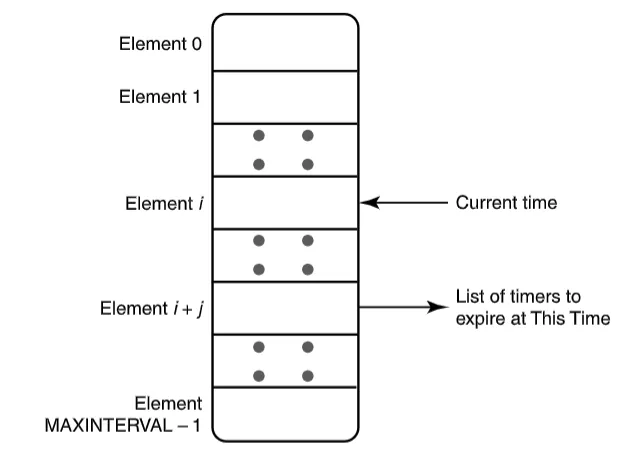
\includegraphics[width=0.8\textwidth]{../assets/ch01/ch01-1_5_端_定时器-001.png}
\end{figure}
图7.1用于说明方案2的定时器队列示例
在第二种简单方案中（用于UNIX的旧版本），PERTICKBOOKKEEPING的延迟降低了，但这是以
STARTTIMER的性能为代价的。定时器存储在一个有序列表中。与方案1不同，我们将存储定时器到期的
绝对时间，而不是到期前的间隔时间。最早到期的定时器存储在列表的头部。后续的定时器按递增顺序
存储，如图7.1所示。在图7.1中，最早到期的定时器将在绝对时间10小时23分12秒到期。



由于列表是排序的，PERTICKBOOKKEEPING只需要增加当前时钟时间，并将其与列表头部进行比较。
如果两者相等，或者当前时间大于列表头部的时间，它就会删除该列表元素，并调用
EXPIRYPROCESSING。它会继续删除列表头部的元素，直到列表头部的到期时间严格小于当前时间。
STARTTIMER通过搜索列表来找到插入新定时器的位置。在示例中，STARTTIMER将把一个在10:24:01
到期的新定时器插入到第二个和第三个元素之间。
                                                        4
启动定时器的最坏情况延迟是O(n)。平均延迟取决于定时器间隔（从开始时间到停止时间）的分布以及
调用STARTTIMER的到达过程的分布。
如果列表是双向链表，STOPTIMER就不需要搜索列表。当STARTTIMER将一个定时器插入到有序列表
中时，它可以存储一个指向该元素的指针。然后STOPTIMER可以使用这个指针在O(1)时间内从双向链表
中删除该元素。这可以应用于任何定时器方案。这是P9原则（在层接口中传递提示）的一个应用。更准
确地说，用户在STOPTIMER接口中向定时器传递一个句柄。
如果这个方案由主机处理器实现，并且有硬件支持来维护单个定时器，那么每次滴答时的中断开销就可
以避免。硬件定时器被设置为在列表头部的定时器到期时到期。硬件会拦截所有时钟滴答，只有当定时
器实际到期时才会中断主机。不幸的是，一些处理器架构不提供这种能力。
在空间方面，方案1需要尽可能少的空间；方案2需要O(n)的额外空间来存储队列元素之间的前向和后向
指针。
链表是实现优先级队列的一种方式。对于较大的n，基于树的数据结构更好。这些数据结构包括非平衡二
叉树、堆、后序和终序树以及左偏树（Cormen等人，1990；Vaucher和Duval，1975）。它们试图将方
案2中STARTTIMER的延迟从O(n)降低到O(log(n))。在Myhrhaug（2001）中报告称，对于较大的n，这
种差异是显著的，并且非平衡二叉树比平衡二叉树成本更低。
不幸的是，非平衡二叉树很容易退化为线性列表；例如，如果插入一组相等的定时器间隔，就会发生这
种情况。不过，将时间轮的性能与使用简单二叉堆的实现进行比较是个好主意。我们将这些算法归为方
案3：基于树的算法。Linux高分辨率定时器（hrtimers）使用平衡（红黑）树（Gleixner和Niehaus，
2006）。
因此，这三种简单方案在STARTTIMER或PERTICKBOOKKEEPING操作中，花费的时间至少与定时器数
量成对数关系。这对于高速实现来说是个问题。下一节将展示如何做得更好。
7.4 时间轮
第一种方案的设计遵循一种常见的问题解决范式：先解决一个更简单的问题，然后利用从中获得的见解
来解决更复杂的问题。
我们首先处理的更简单问题如下。假设所有定时器都设置为某个较小的间隔，例如MAXINTERVAL，并
且假设定时器的粒度为1个时间单位。这表明可以使用P4原则（桶排序技术），而不是方案2和方案3中建
议的排序技术。然而，桶排序实际上用于对一组数字进行静态排序。在这里，新的数字不断被添加和删
除，而我们仍然希望保持顺序。（从技术算法角度来说，定时器数据结构必须实现一个优先级队列，支
持添加、删除和查找最小元素的操作。）与优先级队列等价的桶排序是什么呢？
基于这个动机，不难让读者脑海中浮现出以下画面（如\begin{figure}[htbp]
\centering
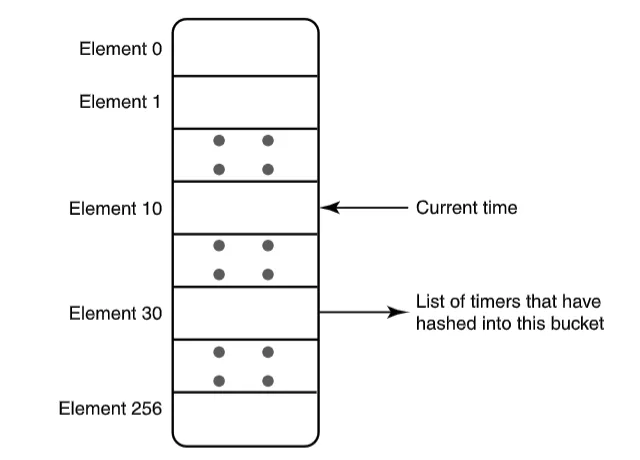
\includegraphics[width=0.8\textwidth]{../assets/ch01/ch01-1_5_端_定时器-002.png}
\end{figure}
图7.2所示）。想象当前时间由一个指向循环数组
中某个元素的指针表示，该循环数组的维度为[0, MAXINTERVAL - 1]。在每次定时器滴答（用于每滴答
记账）时，我们只需将指针增加1，并对数组大小取模。
                                                             5
图7.2方案4用于最大间隔为MAXINTERVAL的定时器的列表数组
要设置一个在当前时间之后j个时间单位到期的定时器，我们对元素(i + j) mod MAXINTERVAL进行索引
（见图7.2），并将定时器放在一个定时器列表的头部，该列表中的定时器将在时间 = 当前时间 + j个时
间单位时到期。每次滴答时，我们递增当前定时器指针（对MAXINTERVAL取模），并检查指针指向的
数组元素。如果该元素为0（没有等待到期的定时器列表），那么在该定时器滴答时就不再进行其他工
作。但是，如果该元素不为零，那么我们对存储在该列表中的所有定时器执行EXPIRYPROCESSING。
因此，STARTTIMER的延迟为O(1)；除了定时器到期时，PERTICKBOOKKEEPING的延迟也是O(1)，但
这已经是最好的情况了。如果定时器列表是双向链表，并且和之前一样，我们为每个定时器记录存储一
个指针，那么STOPTIMER的延迟也是O(1)。
我们可以更形象地将这个数组描述为一个时间轮，其中时间轮每个定时器单位转动一个数组元素。对于
秘书来说，这类似于到期提醒文件。对于排序专家来说，这类似于用空间换处理效率的桶排序。然而，
由于定时器的值随时都在变化，时间间隔是相对于当前时间指针的偏移量。只要当前时间指针随时递增
就足够了。
桶排序使用M个桶在O(M)时间内对N个元素进行排序，因为需要检查所有的桶。对于较大的M > N，这是
低效的。然而，在定时器算法中，关键的观察结果是，某个实体需要每滴答执行O(1)的工作来更新当前时
间；对于同一个实体来说，遍历一个空桶只需要多执行几条指令。这是使用P4原则（利用系统组件）和
P2c原则（费用分摊）的一个很好的例子。
系统已经在每滴答执行一些工作来增加时间。因此，在计算算法成本时，重要的是算法带来的额外开
销，而不是像在算法课上通常测量的那样单独计算成本。请注意，如果系统不是在每个时钟滴答都执行

                                                           6
一些工作，而是依赖于一块硬件来保持时间，那么这个假设就不成立。与排序不同，重要的不是对N个元
素进行排序的总工作量，而是每个定时器滴答需要执行的平均（和最坏情况）工作量。
然而，内存是有限的：很难为了实现32位定时器而分配2^32个字的内存。那么如何将这个想法扩展到更
大的定时器值呢？如果你之前没有接触过这个问题，在继续阅读之前，试着自己想出一些办法。
一种简单的解决方案是在给定的内存范围内使用这个方案来实现定时器。对于大于这个范围的定时器
值，可以使用其他方案，比如方案2。或者，这个方案可以通过两种方式进行扩展，以便在使用适量内存
的情况下支持更大的定时器间隔值。这两种技术的灵感来自两种算法技术（P15）：哈希和基数排序。
7.5 哈希轮
系统已经在每个时钟周期做了一些增加时间的工作。因此，在计算算法成本时，重要的是算法带来的额
外开销，而不是像在算法课上通常单独测量的成本。需要注意的是，如果系统不是在每个时钟周期都做
一些工作，而是依靠一块硬件来记录时间，那么这个假设就不成立。与排序不同，重要的不是对N个元素
进行排序的总工作量，而是每个定时器时钟周期需要完成的平均（以及最坏情况）工作量。
然而，内存是有限的：很难为了实现32位定时器而分配 232 个字的内存。那么，如何将这个想法扩展到
更大的定时器值呢？如果你之前没有接触过这个问题，在继续阅读之前，不妨先尝试自己思考一下解决
方案。
一种简单的解决方法是，在给定的内存和方案下，实现一定范围内的定时器。对于大于这个范围的定时
器值，可以采用其他方案，比如方案2。另外，这个方案可以通过两种方式进行扩展，以便在使用适量内
存的情况下支持更大的定时器间隔值。这两种技术的灵感来源于两种算法技术（P15）：哈希和基数排
序。
7.5 哈希轮
第一种扩展的设计遵循了第二种常见的问题解决范式：通过类比，从不同问题的解决方案中推导出解决
当前问题的技术。
许多想法最初都是通过类比产生的，尽管类比并不总是完全准确。前面的方案与使用元素值作为索引在
数组中插入元素有明显的相似之处。如果内存不足，我们可以对元素值进行哈希运算以得到一个索引
吗？例如，如果哈希表的大小是2的幂次方，那么任意大小的定时器值都可以很容易地除以哈希表大小；
余数（低阶位）与当前时间指针相加，得到数组中的索引。除法的结果（高阶位）则存储在由该索引指
向的列表中。
在\begin{figure}[htbp]
\centering
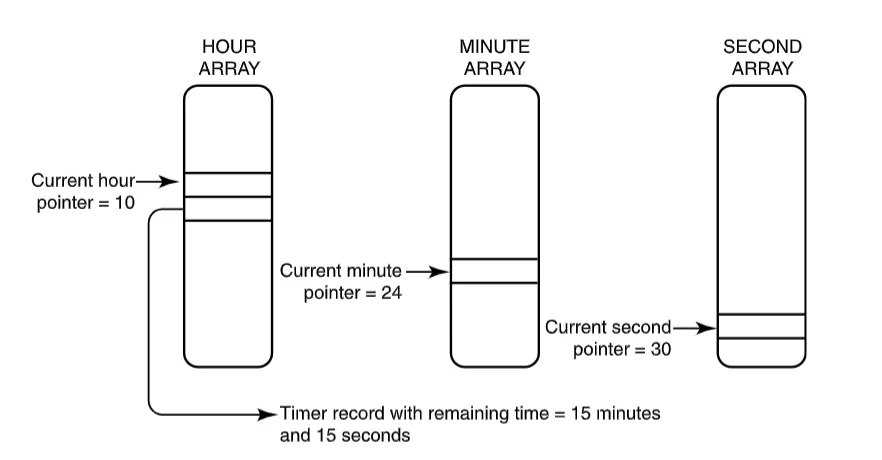
\includegraphics[width=0.8\textwidth]{../assets/ch01/ch01-1_5_端_定时器-003.png}
\end{figure}
图7.3中，假设哈希表大小为256，定时器为32位定时器。除法的余数是最后8位。假设最后8位的值为
20。那么定时器的索引就是10（当前时间指针） + 20（余数） = 30。然后，将24个高阶位插入到由第
30个元素指向的列表中。

                                                    7
也可以使用其他哈希方法。例如，可以使用任何将定时器值映射到数组索引的函数。我们将在7.5节末尾
阐述选择这种方法的理由。然而，现在我们的设计面临一个分歧点。无论使用哪种哈希函数，都有两种
维护每个列表的方式。
最直接的方法（在深入研究之前，这似乎是最好的方法）是在每个桶内采用方案2。这显然是对方案2的
扩展，同时提高了其性能，因为每个 “小” 列表应该比单个列表小。现在来详细说明一下。不幸的是，它
的性能取决于哈希函数，因为STARTTIMER操作可能会很慢，原因是24位的数量必须插入到列表中的正
确位置。因此，STARTTIMER的最坏情况延迟仍然是 O(n) 。
假设 O(n) 的STARTTIMER最坏情况延迟是不可接受的，我们可以将每个时间列表维护为无序列表，而
不是有序列表。乍一看，这似乎是个糟糕的主意。我们确实使STARTTIMER操作更快了；但是，如果列
表是无序的，那么每个时钟周期似乎都需要做更多的工作，这似乎是一个糟糕的权衡。不过，让我们再
仔细分析一下。
显然，STARTTIMER现在的最坏情况和平均延迟都是 O(1) 。PERTICKBOOKKEEPING操作现在确实
花费的时间更长。每个定时器时钟周期，我们递增指针（对TableSize取模）；如果那里有一个列表，我
们必须像在方案1中那样，对数组中的每个元素的高阶位进行递减操作。然而，如果哈希表具有前面描述
的属性，那么列表的平均大小将是 O(1) 。
无论哈希函数如何分布，我们都可以对平均情况做出更强的说明。这可能不是那么显而易见。请注意，
每经过TableSize个时钟周期，我们就会对所有仍然有效的定时器递减一次。因此，对于n个定时器，我
们每个时钟周期平均执行 n/T ableSize 的工作量。如果 n < T ableSize ，那么我们每个时钟周期
平均执行 O(1) 的工作量。如果所有n个定时器都哈希到同一个桶中，那么每经过TableSize个时钟周
期，我们执行 O(n) 的工作量，但在中间的时钟周期，我们执行 O(1) 的工作量。这意味着，如果我
们希望保持每个时钟周期的工作量小且有界，我们只需确保桶的数量比我们支持的最大并发定时器数量
大一定倍数。我们甚至可以通过增加桶的数量来尽可能地减少这项工作。这是一个关于分摊复杂度的例
子，它比关于平均复杂度的结果更强。
因此，方案6中的哈希分布只控制PERTICKBOOKKEEPING延迟的 “突发性”（方差），而不控制平均延
迟。由于PERTICKBOOKKEEPING的最坏情况延迟始终是 O(n) （所有定时器同时到期），我们认为
方案6中哈希函数的选择并不重要。通过除以2的幂次方取余数的方法成本较低，因此推荐使用。此外，
使用任意哈希函数将定时器值映射到数组索引，会要求PERTICKBOOKKEEPING在每个定时器时钟周期
计算哈希值，这将使其成本更高。




                                                          8
图7.3方案5和方案6用于任意大小定时器的列表数组：基本是一个哈希表
7.6 分层轮




\begin{figure}[htbp]
\centering
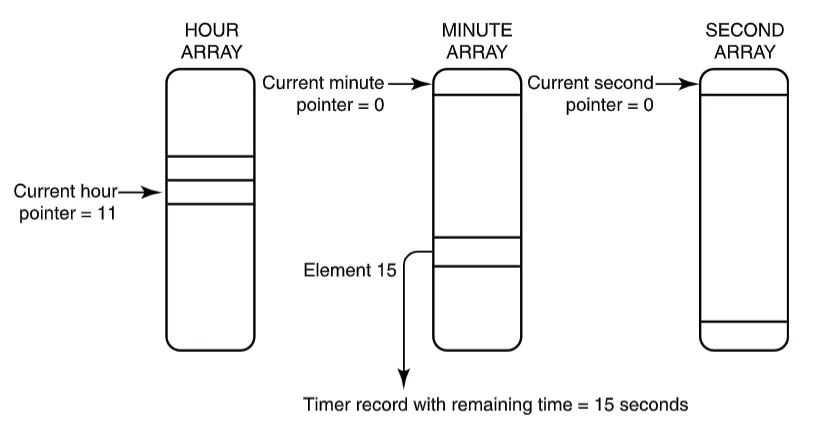
\includegraphics[width=0.8\textwidth]{../assets/ch01/ch01-1_5_端_定时器-004.png}
\end{figure}
图7.4方案7使用的分层列表数组，用于更高效地 “映射” 时间
7.6 分层轮
基本方案的第二种扩展利用了分层的概念。为了表示数字1000000，我们只需要7位数字，而不是
1000000个数字，因为我们以1、10、100等为单位分层表示数字。同样，为了表示32位范围内的所有可
能定时器值，我们不需要一个有 232 个元素的数组。相反，我们可以使用多个不同粒度的数组。例如，
我们可以使用以下四个数组：
  ● 一个有100个元素的数组，每个元素代表一天；


                                                   9
 ●  一个有24个元素的数组，每个元素代表一小时；
  ● 一个有60个元素的数组，每个元素代表一分钟；
  ● 一个有60个元素的数组，每个元素代表一秒。

因此，要存储长达100天的定时器，我们不需要 100 × 24 × 60 × 60 = 864 万个存储位置，而只需要
 100 + 24 + 60 + 60 = 244 个位置。
例如，看图7.4。假设当前时间是11天10小时24分30秒。要设置一个50分钟45秒的定时器，我们首先计
算定时器到期的绝对时间，即11天11小时15分15秒。然后，我们将定时器插入到小时数组中，位于当前小
时指针（10）向前1（11 - 10小时）个元素的列表中。我们还将余数（15分钟15秒）存储在这个位置。在
图7.4中展示了这一过程，为简化示例，忽略了在该示例中未发生变化的日期数组。
秒数组的工作方式与通常一样：每次硬件时钟滴答时，我们递增秒指针。如果该元素指向的列表不为
空，我们对列表中的元素执行EXPIRYPROCESSING操作。然而，其他三个数组的工作方式略有不同。
即使服务的用户没有请求任何定时器，也总会有一个60秒的定时器用于更新分钟数组，一个60分钟的定
时器用于更新小时数组，以及一个24小时的定时器用于更新日期数组。例如，每次60秒定时器到期时，
我们将递增当前分钟定时器，对分钟定时器执行任何必要的EXPIRYPROCESSING操作，并重新插入另
一个60秒定时器。
回到前面的例子，如果定时器未停止，最终小时定时器将到达11。当小时定时器到达11时，会检查列表；
EXPIRYPROCESSING将把剩余的秒数（15）插入到分钟数组中，位于当前分钟指针（0）之后的第15个
元素处。当然，如果剩余分钟数为零，我们可以直接进入秒数组。此时，表格看起来将如\begin{figure}[htbp]
\centering
\includegraphics[width=0.8\textwidth]{../assets/ch01/ch01-1_5_端_定时器-005.png}
\end{figure}
图7.5所示。




图7.5前一个例子，但在定时器的小时部分到期后（使用方案7）
最终，分钟数组将到达第15个元素；作为EXPIRYPROCESSING的一部分，我们将把定时器移动到秒数
组中，位于当前值之后的15秒处。15秒后，定时器将实际到期，此时将执行用户指定的
EXPIRYPROCESSING操作。

                                                         10
在方案6和方案7之间做出选择并不容易。对于较小的T值和较大的M值，方案6在STARTTIMER和
PERTICKBOOKKEEPING操作上可能都比方案7更好。然而，对于较大的T值和较小的M值，方案7在
PERTICKBOOKKEEPING的平均成本（延迟）方面会更好，但在STARTTIMER延迟方面成本更高。
需要注意的是，如果允许定时器的精度随着分层级别增加而降低，那么我们就不需要在不同级别之间迁
移定时器。例如，在前面的例子中，我们可以将时间四舍五入到最接近的小时，只设置小时级别的定时
器。当小时定时器到期时，我们执行用户指定的EXPIRYPROCESSING操作，而无需迁移到分钟数组。
本质上，我们现在有了不同的定时器模式，一种用于小时定时器，一种用于分钟定时器，等等。这进一
步降低了PERTICKBOOKKEEPING的开销，但代价是精度损失高达50%（例如，一个1分30秒的定时器
被四舍五入为1分钟）。或者，我们可以通过允许在相邻列表之间仅进行一次迁移来提高精度。
7.7 BSD实现
目前，Linux内核针对本章开头描述的两种不同用例，提供了两种不同的定时器设施。高分辨率定时器
（“hrtimer”）机制为用户提供精确的定时器，这些定时器会运行至完成，例如在速率控制算法中使用。
较低分辨率的定时器用于事件超时和故障推断。虽然高分辨率定时器使用平衡（红黑）树（Gleixner和
Niehaus，2006），但较低分辨率的定时器（Corbet，2015）使用分层定时器，不过，如前所述，它选
择限制定时器迁移（在Linux术语中称为 “级联”（Corbet，2015）），以牺牲精度为代价。早期版本的
Linux（1997年首次实现（Gleixner和Niehaus，2006））只使用了一种方法 —— 带有迁移的分层时间
轮，称为级联时间轮（CTW）。
7.7 BSD实现
Adam Costello率先使用哈希轮实现（Costello和Varghese，1998）了BSD UNIX的调用和定时器设施。
早期的BSD内核在设置或取消定时器时所花费的时间与未完成定时器的数量成正比。而基于方案6的
Costello实现，启动、停止和维护定时器的时间是恒定的；这带来了高度可扩展的设计，能够轻松支持数
千个未完成的定时器，且开销很小。
在最初的BSD实现中，每个调用由一个CALLOUT结构表示，该结构包含一个指向要调用函数的指针
（C_FUNC）、一个指向函数参数的指针（C_ARG），以及一个以时钟滴答为单位表示的时间
（C_TIME）。未完成的调用存储在一个链表中，并根据到期时间进行排序。每个CALLOUT结构的
C_TIME成员是相对时间，而不是绝对时间；链表中的第一个调用存储从现在到到期的滴答数，后续每个
调用存储其自身到期时间与前一个调用到期时间之间的滴答数。
在BSD UNIX中，调用分别使用TIMEOUT()和UNTIMEOUT()来设置和取消。TIMEOUT(FUNC, ARG,
TIME)注册FUNC(ARG)在指定时间被调用。UNTIMEOUT(FUNC, ARG)取消具有匹配函数和参数的调
用。由于对CALLTODO列表进行线性搜索，最初这两个操作所花费的时间都与未完成调用的数量成正
比。在搜索期间，中断被锁定。

                                                               11
在现有系统中添加新算法有时会遇到与现有接口的兼容性问题。例如，Costello实现基于方案6。然而，
Costello发现，BSD中的TIMEOUT()/UNTIMEOUT()接口不允许传递句柄，而在我们上面描述的所有方
案中，传递句柄用于快速取消定时器。Costello实现通过两种解决方案来解决这个问题。对于使用现有接
口的调用，通过哈希表根据函数指针和参数搜索调用。还实现了第二种解决方案：定义了一个新的接口
函数UNSETCALLOUT()，用于删除调用，该函数仅接受一个句柄作为参数。这使得现有代码可以使用旧
接口，而新应用程序可以使用新接口。这两种方法的性能差异很小，因此哈希表方法更受青睐。
在Costello实现中，定时器例程保证仅在一小段有界时间内锁定中断。Costello实现还扩展了
SETITIMER()接口，允许一个进程拥有多个未完成的定时器，从而减少了用户维护自己定时器包的需求。
对BSD内核的更改很小（添加了548行代码，删除了80行代码）。详细信息可在（Costello和
Varghese，1998）中找到；书面报告包含了一些此处未提及的重要实现细节。
多核机器的出现要求对Costello实现进行更改。早期的一项更改是，将单个调用轮替换为每个CPU一个
调用轮，以提高可扩展性和性能（Motin和Italiano，2018）。Motin和Italiano（Motin和Italiano，
2018）最近推出了一个更新版本，称为Calloutng，以解决Costello实现的以下三个缺点。第一，时间间
隔会舍入到下一个时钟滴答，导致精度损失；第二，每次中断都会唤醒CPU，导致额外的能源消耗；第
三，无法延迟和合并调用，从而导致额外的中断。他们考虑过使用平衡树，但最终决定保留轮结构。不
过，代码进行了更新，更加注重精度，允许聚合，使用新的哈希函数对轮进行索引，并仔细考虑了CPU
缓存亲和性的影响（Motin和Italiano，2018）。
7.8 谷歌Carousel实现
在Costello实现多年后，谷歌构建了一个可扩展的流量整形系统，称为Carousel（Saeed等人，
2017），其底层数据结构是一个时间轮，能够处理数十万个并发的细粒度定时器。由于其速度和规模比
Costello实现高得多，我们简要回顾一下推动这种设计的新用例。
第一个用例是在基于速率的拥塞控制算法（如BBR（Cardwell等人，2017））中使用精细的速率调整。
回想一下，TCP拥塞控制算法是基于拥塞信号（如拥塞路由器设置的拥塞标志位和丢弃的数据包）来减
小窗口大小（未确认的字节数）。TCP拥塞控制算法的问题在于，当收到大量字节的累积确认时，发送
方可能会向网络中突发大量流量，这可能导致路由器丢弃数据包。相比之下，基于速率的拥塞算法（如
BBR）根据拥塞信号控制数据包的发送速率。而速率又由精细的定时器控制，这些定时器控制数据包发
送之间的时间间隔。据报道，使用BBR大大改善了全球的往返延迟和YouTube的体验质量指标
（Cardwell等人，2017）。
第二个用例是在服务器中实现虚拟机（VM）隔离，这些服务器托管着数千个虚拟机，每个虚拟机可以与
数百个其他虚拟机进行通信。如果不对每个虚拟机单独或总体使用的带宽进行限制，一旦某个虚拟机以
过高的速率发送数据，其他虚拟机可能会受到不利影响，因为它们共享相同的物理出站链路。第三个用
例与数据中心计算中的Incast问题（Saeed等人，2017）类似，在这种情况下，一个请求会收到来自其他

                                                                12
服务器的数百个响应，这会导致路由器丢弃数据包。通过让繁忙的接收方使用精细的速率调整来控制其
发送回的确认消息，可以缓解Incast问题。
第二个和第三个用例传统上是通过令牌桶方案来实现的，我们将在关于路由器QoS的第14章中描述该方
案。简而言之，其思想是为每个用户分配一定数量的令牌，用户在每个定时器时钟周期可以使用这些令
牌发送字节数。当用户发送的字节数超过其拥有的令牌数时，用户的流量要么被丢弃（在这种情况下称
为策略器），要么被放入队列中，直到有更多令牌到达（在这种情况下称为整形器）。虽然这种方案传
统上在路由器中实现，但上述三个用例需要在主机中使用令牌桶。例如，Linux的流量控制组件Qdisc
（Components of Linux Traffic Control）支持不同的公平队列策略，包括HTB（hierarchical token
buckets）。
对谷歌服务器的测量（Saeed等人，2017）表明，在Linux中使用现有的Qdisc机制，要么导致速率控制
不完善，要么造成过高的CPU开销。因此，Carousel的设计者（Saeed等人，2017）没有依赖Linux的定
时器，而是采用了大型哈希时间轮。 然而，Carousel并非定时器工具，而是一种能够扩展到处理数十万
个流量的流量整形器/策略器。为避免流量整形器中出现应用程序持续突发数据包并在Carousel中排队的
问题，Carousel系统还引入了一种称为延迟完成的概念。 延迟完成的理念是，在Carousel将存储的数据
包发送到网卡之前，不允许系统调用完成。这就提供了一种反馈机制，能够让过于激进的发送方降低发
送速度。延迟完成意味着完成情况可能会乱序到达 —— 一个速率设定较慢的应用程序，即便其请求发送
得更早，却可能比速率较快的应用程序更晚收到完成通知。这就需要使用哈希表（P15）来匹配完成情况
和请求，虽然增加了复杂性，但却很有价值。因此，延迟完成是一种更改接口的方式（P9）。 需要注意
的是，与传统使用定时器来触发重传或检测故障的场景不同，Carousel中的定时器总是会到期（不像重
传定时器或故障检测定时器，它们几乎不会到期），所以Linux定时器工具中采用的一些优化方法（见
Corbet，2015）无法在Carousel中使用。相反，Carousel采用了其他几种实现技巧。Carousel为每个
CPU配备一个时间轮，以避免锁竞争，并且在必要时可以利用多个内核。它还使用预分配缓冲区
（P2a）来降低缓冲区分配的开销。 最终结果是，Carousel对谷歌流量的整形精度比早期最好的流量整
形技术提高了10倍（Saeed等人，2017），同时将整体机器的CPU利用率提高了10%，内存使用量相比
早期技术降低了两个数量级。这表明，将时间轮从根本上融入到流量整形算法中（而不仅仅作为定时器
工具使用），再结合延迟完成等创新技术，能够发挥巨大的作用。
7.9 获取更细粒度的定时器
随着网络速度的提升，人们可能会认为，随着到目的地的往返延迟减少，重传定时器的时长也会相应缩
短。如果往返延迟降至微秒级别，那么重传定时器也降至微秒级似乎是合理的。但遗憾的是，在大多数
操作系统中，即便往返延迟已降至微秒级，人们仍只能使用毫秒级的定时器。虽然时间轮的使用能够实
现更细粒度的重传定时器，但定时器的粒度仍然无法小于定时器的时钟周期。
如今，许多CPU都配备了可编程的硬件中断芯片，可将其编程为以所需频率中断CPU。因此，一种看似
简单的提高定时器分辨率的方法是增加时钟中断的频率。结合时间轮的使用，这似乎能够提供更细粒度
的定时器。
                                                                       13
然而，这个方法存在一个缺陷。正如我们在模型部分所讨论的，现代CPU为了加快处理速度会保存大量
状态信息，这其中包括流水线状态、大量寄存器的使用，以及缓存和页表缓存（TLB）。中断会带来高
昂的开销，因为它涉及到CPU状态的保存和恢复，并且可能会改变局部性模式，导致在退出中断处理程
序后出现缓存和TLB缺失的情况。Aron和Druschel在1999年进行的早期测量表明，在300或500MHz的
奔腾处理器上，一次中断的成本约为4.5微秒。更糟糕的是，随着处理器速度的提升，并没有迹象表明中
断处理时间会有所改善。
因此，更频繁的硬件中断会导致过多的开销。就目前定义的问题而言，如果将定时器模块视为一个黑
盒，我们似乎找不到解决方案。不过，系统思维通过再次考虑P4原则并利用其他系统组件，为我们的困
境提供了解决方案。要知道，CPU的运行过程中充满了其他类型的转换事件，这些事件涉及到状态的保
存和恢复以及局部性模式的改变。这类转换事件包括系统调用（例如，对设备驱动程序的调用）、异常
（例如，页面错误）以及硬件中断（例如，来自网络适配器的中断）。
如果我们将检查过期定时器作为这类转换事件代码的一部分，那么状态保存和局部性改变的开销已经包
含在转换事件中，不会因定时器处理程序而显著增加。这是有利的一面。但不幸的是，与硬件时钟中断
不同，转换事件的频率是不可预测的。这是不利的一面。
不过，Aron和Druschel在1999年对广泛的基准测试进行的实验表明，转换事件之间的平均延迟在5到30
微秒之间，具体取决于CPU正在运行的任务；延迟超过100微秒的情况仅占6%，并且最大延迟从未超过1
毫秒。
这些数据表明了P3原则的一种有趣应用，即放宽系统要求。我们不再提供总是能提供微秒级定时器的
“硬” 定时器设施，而是提供一种 “软” 定时器（Aron和Druschel，1999）设施，它通常能提供10微秒的
定时器。我们还可以通过每1毫秒添加一次硬件时钟中断来限制软定时器设施的误差。因此，软定时器对
于那些能从预期情况（P11）下几十微秒的定时以及最坏情况下1毫秒的定时中受益的应用程序来说是有用
的。
幸运的是，大多数使用定时器的应用程序都能从这种近似定时器中受益。以故障恢复中的快速重传为
例，如果除了偶尔的一次重传需要1毫秒外，大多数重传都很快，那么故障恢复性能将会得到提升。再考
虑控制某些实体产生速率的算法，只要算法的正确性能够容忍速率的变化或抖动，那么在预期情况下性
能应该会有所提高。例如，Aron和Druschel在1999年展示了如何通过速率控制使TCP连接大致每12微秒
发送一个数据包。更精细的速率控制减少了数据的突发性，但速率的偏差并不影响其正确性。
最后，或许处理微秒甚至纳秒级定时器的正确方法是添加硬件（P5）。这种硬件可以是一个定时器芯
片，它使用时间轮或d -堆在芯片内部完全处理所有定时器。这样，芯片内部有一个硬件时钟，硬件时钟
中断在芯片内部处理；只有当定时器到期时，CPU才会被中断。然而，如果定时器经常被取消，CPU与
芯片通信以取消定时器可能会带来相当大的开销。
7.10 结论

                                                        14
本章介绍了两种高效实现定时器的技术。第一种技术是时间轮，它将定时器实现的开销降低到恒定时
间，而与未完成定时器的数量无关。这使得定时器设施能够提供大量定时器，对于如今的互联网服务器
而言，这是一个非常有用的特性，因为这些服务器有时需要为数千个并发客户端提供服务。第二种技术
是软定时器，它减少了PERTICKBOOKKEEPING操作所带来的操作系统开销。这使得定时器设施在预期
情况下能够提供细粒度的定时器，随着互联网链路速度的提升，这一特性非常实用。这两种方案所使用
的原理总结在表7.1中。
当时间轮在1987年首次被提出（Varghese和Lauck，1987）时，人们普遍认为它解决的是一个无关紧要
的问题。正如当时一位系统设计师所说：“如果它没坏，为什么要修呢？”——这是一个合理的问题。然
而，思考那些你预测未来可能出现的问题的解决方案是很有帮助的。以下信息改编自Justin Gibbs
（FreeBSD早期的关键实现者之一）的言论，不过其中关于实际产品使用的内容有些过时。
在本书第一版中引用了Gibbs的话，他说在那个时候，雅虎通过分布在全球的500台FreeBSD服务器提供
所有内容服务。同样在那个时候，最大的基于网络的电子邮件服务提供商Hotmail最初在电子邮件路由和
网络服务中都使用了FreeBSD。此外，包括美国两家最大的互联网服务提供商Best Internet和USWest在
内的数千家互联网服务提供商，在那个时代都依赖FreeBSD为用户提供互联网新闻服务、数据包路由、
网站托管和shell服务。
然而，在1997年下半年，情况变得很明显，FreeBSD内核中使用的定时器服务很快将成为系统吞吐量的
瓶颈。定时器事件被用于多个需要基于事务的时间通知的应用程序中。随着事务数量和 / 或频率的增
加，定时器接口的负载呈线性增长。例如，FreeBSD内核过去会为每个磁盘事务安排一个 “看门狗” 定时
器，如果定时器触发，就会启动错误恢复操作。在一台典型的服务器上，在250个并发磁盘事务的适度负
载下，超过15% 的CPU资源被定时器事件调度所占用。对旧定时器接口所采用算法的分析表明，CPU负
载会随着并发事务数量的增加而线性上升，这损害了系统的可扩展性。
Justin Gibbs在发现并修复了Costello实现中的一个错误后，在FreeBSD中实现了哈希轮。他的实现将
FreeBSD基准测试中的定时器开销降低到了总CPU使用率的一小部分。Costello算法确保了无论事务负
载如何，开销都接近恒定，保证了定时器设施能够轻松扩展以处理数千个事务。虽然BSD代码后来针对
多核机器进行了更新，并且Motin和Italiano在2018年也进行了进一步更新，但二十年后，哈希轮的基本
用法仍然存在。
许多其他操作系统，如Linux，现在也使用时间轮，大多数实时操作系统（包括路由器中使用的操作系
统）也是如此。需要注意的是，Linux提供了两种定时器设施：一种是粗粒度定时器（Corbet，2015），
它使用分层时间轮，但限制了时间轮之间的迁移（在Linux术语中称为 “级联”）；另一种是高分辨率定
时器（Gleixner和Niehaus，2006），它使用红黑树。最后，现代云操作系统在对数十万个流量进行非
常精细粒度的可扩展流量整形时，也使用哈希轮，因为哈希轮能够在低CPU开销的情况下实现更精确的
流量整形（Saeed等人，2017）。从长远来看，关注算法设计是会有回报的。



                                                        15
